\documentclass[a4paper, 10pt, conference]{ieeeconf}
\IEEEoverridecommandlockouts
\overrideIEEEmargins

\usepackage{graphics} % for pdf, bitmapped graphics files
\usepackage{epsfig} % for postscript graphics files
\usepackage{mathptmx} % assumes new font selection scheme installed
\usepackage{times} % assumes new font selection scheme installed
\usepackage{amsmath} % assumes amsmath package installed
\usepackage{amssymb}  % assumes amsmath package installed
\usepackage{multirow}  % assumes amsmath package installed
\usepackage{float}  % assumes float package installed
\usepackage{upgreek}  
\usepackage{tabularx}  
\usepackage{epstopdf}
\usepackage{caption}
\usepackage{subcaption}
\usepackage{wrapfig}

\title{\LARGE \bf Using CRFs for Rover Locomotion Diagnosis}

\author{Christian Vassallo, Karthick Munirathinam (???), Sophie Sakka, Christine Chevallereau 
\thanks{This work was supported by IRCCyN Robotics Lab and WILLPOWER scholarship}% <-this % stops a space
\thanks{christian.vassallo@laas.fr, K. Munirathinam, S. Sakka and C. Chevallereau are with IRCCyN, Nantes, France
        {\tt\small karthick.munirathinam@irccryn.ec-nantes.fr sophie.sakka@irccryn.ec-nantes.fr christine.chevallereau@irccryn.ec-nantes.fr}}%
\thanks{Sophie Sakka is also with University of Poitiers, France}%
}

\begin{document}

\maketitle
\thispagestyle{empty}
\pagestyle{empty}


%%%%%%%%%%%%%%%%%%%%%%%%%%%%%%%%%%%%%%%%%%%%%%%%%%%%%%%%%%%%%%%%%%%%%%%%%%%%%%%%
\begin{abstract}
To write.\par
\end{abstract}


%%%%%%%%%%%%%%%%%%%%%%%%%%%%%%%%%%%%%%%%%%%%%%%%%%%%%%%%%%%%%%%%%%%%%%%%%%%%%%%%
\section{Introduction}

To write. \par



%%%%%%%%%%%%%%%%%%%%%%%%%%%%%%%%%%%%%%%%%%%%%%%%%%%%%%%%%%%%%%%%%%%%%%%%%%%%%%%%
\section{Equipment and Human Motion}

In our experiments the human performances are recorded using the marker-based capture system ART - Advance Realtime Tracking system, supplied by DTrack2 and ART-Human software to elaborate the actor movements. The system consists of a hybrid suit of 17 targets with 6 degrees of freedom relative to left/right foot, shin, thigh, shoulder, upper-arm, forearm, hand, head, hip, back and torso.
To record the human movements a set of 8 IR cameras are located in the eight corners of the 3D rectangular work space. The system is able to capture information with different frequencies but we choose to set it at 50 Hz in order to match the motion frequency of the humanoid robot NAO.
The ART software DTrack2 acquires the 2D information of each IR camera and provides the transformation matrices relative to the different local frames attached to the body parts. The origin of each local frame is set to the center of gravity of all markers attached to the relative limb. The axes of the body coordinate system are parallels to the axes of the room coordinate system in the beginning
of the body calibration \cite{GmbH2012}.
ART-Human software uses the information provided by DTrack2 to design each segment limb automatically. During the calibration, it estimates the position and orientation of the actor articulation frames and the limbs dimension are computed as an offset.\\
In the first part we considered simple motion as left kick, starting and ending in double support, and waving motion in double support.
Since the robot and human kinematics are different, during the imitation the balance could be not preserved and the robot may fail down.

\section{Motion Conversion}
The main problem arisen during human to humanoid motion conversion is to find a good compromise between the fidelity and the feasibility of the imitation. The several differences, especially from kinematics point of view, do not allow to obtain a perfect conversion, especially preserving the human style.
The goal is then to capture human movements and observe the robot imitator performing motions apparently identical to the original ones.
In despite of other related researches, in which the conversion algorithm works in joint space, we consider only the Cartesian aspects of the actor movements because we suppose that in this way some particular features, like the human style, are preserved.
Considering the data provided by DTrack2 software, the idea is to define some \textit{Virtual Markers} on the humanoid robot NAO such that during the movements their position and orientation evolution match the \textit{Real Markers} evolution equipped by the actor.
\subsection{Mathematical Formulation of the Problem}
In order to realize our idea, we formulate the following optimization problem in which the cost function is defined as a difference between the Real Marker $\mathit{^{0}T_{m_i}}(t)$ attached to the limb $i^{\,th}$ measured by MoCap and the relative Virtual Marker $\mathit{^{0}T_{V_i}}(q)$ computed recovering the joint angles of the robot. Whole body motion is considered for each instant of time, such that:
\begin{equation}
\sum^{T}_{t=0} \, \sum^{M}_{i=1} \, || \, ^{0}T_{m_i}(t) - ^{0}T_{V_i}(q) ||_2
\label{eq:minimizationReal-Virtual-Marker}
\end{equation}
In the following paper we will represents the objective function in equation \eqref{eq:minimizationReal-Virtual-Marker} as a difference between two transformation matrices.
However, the computation is done in more than one step, following the algorithm described by W. Khalil in \cite{Khalil2002} to solve the inverse geometric problem: firstly, we compute the error vector in position $\mathit{dX_{p_i}}$ and orientation ${\mathit{dX_{r_i}}}$, representing the difference between the desired configuration $^{0}T_{m_i}(t)$ and the current configuration $^{0}T_{V_i}(q)$. Note that $\mathit{dX_{p_i}} =\, ^{0}T_{m_i}(t) - \, ^{0}T_{V_i}(q)$ and ${dX_{r_i}} = \mathbf{u} \cdot \alpha$, where the angle $\alpha$ and the unit vector \textbf{u} are obtained computing $\,^{0}R^T_{V_i}(q) \,^{0}R_{m_i}(t)$.
Successively, the joints configuration $q$ is optimized to minimize the error.

Consequently, the frames virtually attached to the humanoid robot limbs are computed as function of the joints trajectory. Let be $q_0$ and $t_o$ respectively the initial configuration of the robot and the initial instant of time, each Virtual Marker is computed with respect to the relative limbs $i$ ( e.g. Elbow-Forearm, Knee-Shin, Ankle-Foot)as follows:
\begin{equation}
^{0}T_{V_i}(q) = \, ^{0}T_{j}(q_i{_0}) \, \cdot \, ^{j}T_{V_i}
\label{eq:Virtual-Marker-Definition}
\end{equation}
where $^{j}T_{V_i}$ is the relation matrix between the robot joint $j$ and the relative Virtual Marker. Since humanoid system is a rigid body, the relation matrix is considered constant. Each Virtual Marker $V_i$ is uni-vocally related with one joint $j_i$.
 
However, the equation \eqref{eq:minimizationReal-Virtual-Marker} compares the Real Markers on the actor and the Virtual Markers on the robot. Therefore, it is necessary to find a relation between the two systems in order to solve the discrepancies between human actor and robot imitator: 1) different body dimension, 2) different mobility, 3) non-rigid body motion.

\subsection{Human Movements Analysis}
In the first part of our work we analyze the actor movements data, exploiting the functionality of our motion capture system ART that provides information also relative to the actor joints. Considering the same left kicks at three different velocities (slow, medium and fast), we observe the distance variation between two articulation frames relative to the same appendage (e.g. Elbow and Wrist) and the offset between the human joint and the marker on the relative limb $^{j_{i}}P_{V_{i}}$. In all the cases the length of each body part is almost constant (variation less than $1\%$ of total length); nevertheless the distance between the Real Marker and the actor joint frame varies from $15\%$ up to $30\%$ of total length as shown in Figure \ref{fig:distVariation}.
\begin{figure}[b]
		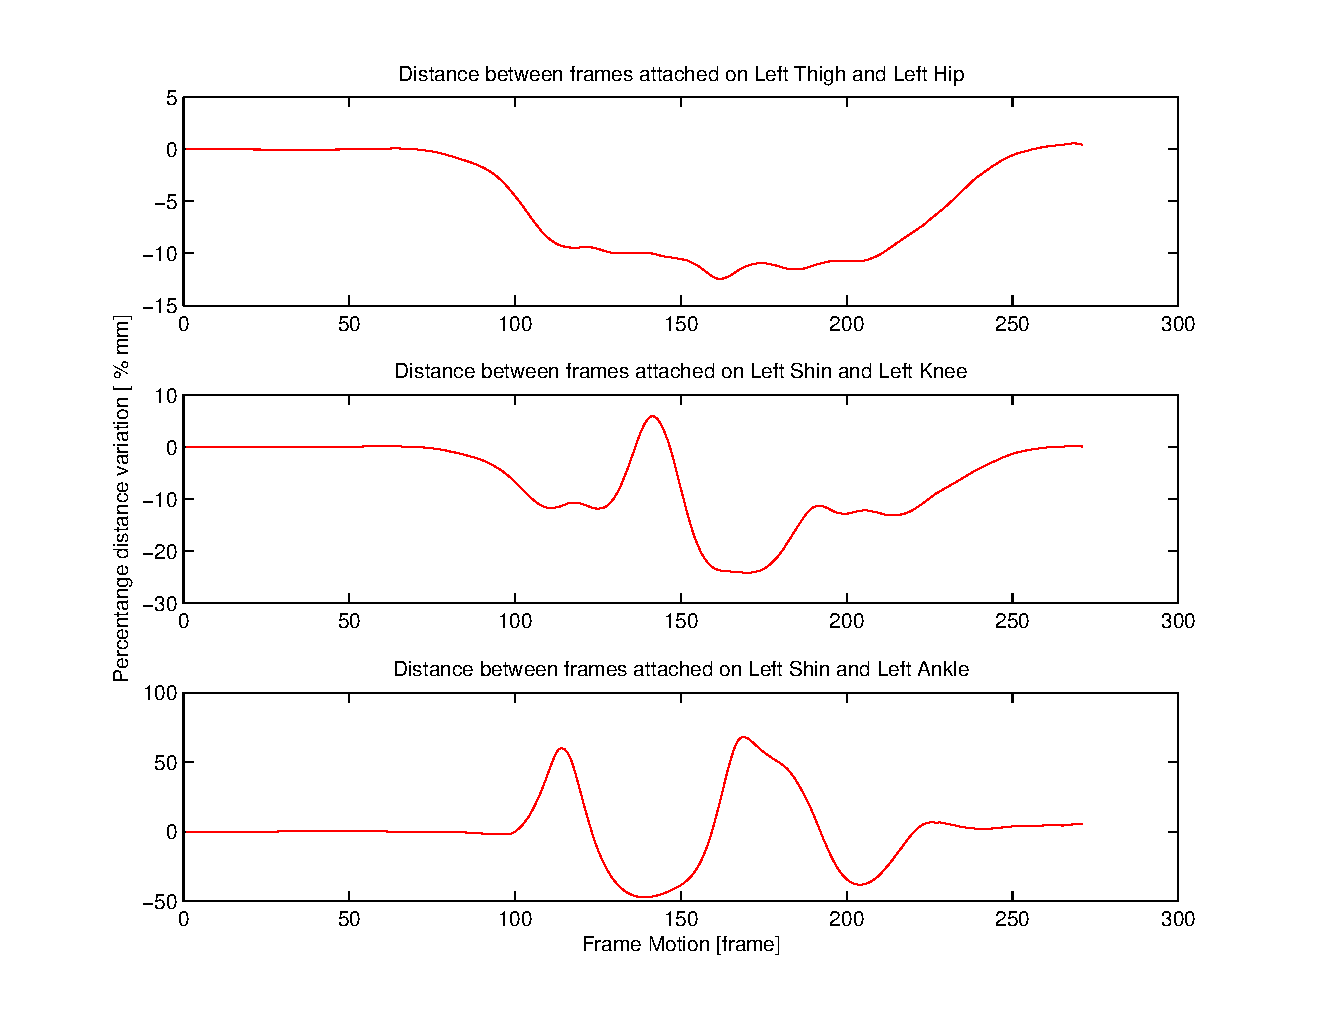
\includegraphics[width=\linewidth]{Figures/distVariation.eps} 
		\caption{Variation of the distance between real markers on the left leg of human actor.}
		\label{fig:distVariation}
\end{figure}
The skin-artifact problem can be reduced equipping as better as possible the actor but it is not physically possible to avoid it completely. Since the noise of the system is in the vicinity of 1-2 mm., it does not influence considerably the results. Ude at al. propose in \cite{Ude2000,Ude2004} to consider an initial configuration for defining the local frames with respect to a global body coordinate system. Taking the cue from their work, we instructed the actor to perform the movements starting from double support in upright position with arms and legs full extended. This configuration is the initial configuration and it is presented as \textit{Zero Body Configuration}.
Thereby we decide to acquire N samples (with $1000 < N < 5000$) of the actor in Zero Body Configuration without motion: the length of each limb is then computed considering the mean value. 

Once defined the body part dimensions, we decide to approximate the actor movements as a rigid body motion and the hypothesis done for the Equation \eqref{eq:Virtual-Marker-Definition} can be considered.
The problem of different body size and mobility can be solved adapting the robot kinematics with the human dimensions.
Some authors as Martin Do \cite{Do2008} propose the Master
Motor Map interface for mapping the human movements to the human-like motion on the humanoid, preserving the features of the original performance.
Our method tries to introduce an easier way for the motion conversion. Basically, the idea consists to apply the body dimensions of the human to the kinematics model of the humanoid robot. In our work we implement this method in the humanoid robot NAO which presents physical characteristics completely different than any actor.
Analyzing Figure \ref{fig:scalingprocess}, it is possible to observe the MATLAB representation of the human model using the information provided by ART-Human software and the model of humanoid NAO in normal and scaled-up version.
One of the problems engaged during the development of the motion conversion algorithm was to define a relation between the humanoid robot NAO reference frame and the motion capture system.
%\begin{figure}[t]
%		\includegraphics[width=\linewidth]{Figures/scalingprocess} 
%		\caption{Actor and NAO robot in Zero Body Configuration. In the right the robot kinematics adapted to the real actor size is represented.}
%		\label{fig:scalingprocess}
%\end{figure}

The criteria in Equation \eqref{eq:minimizationReal-Virtual-Marker} considers the two information expressed with respect to the same reference frame.
Nevertheless, the Real Markers are expressed in the MoCap frame as function of $t$ and the Virtual Markers are expressed in the zero frame of robot NAO as function of $q$.
Therefore, it is necessary to find a relation between the two reference frames such that:
\begin{equation}
\sum^{T}_{t=0} \, \sum^{M}_{i=1} \, || \, ^{0_{MoCap}}T_{m_i}(t) \, - \, ^{0_{MoCap}}T_{0_{NAO}} \, \cdot \, ^{0_{NAO}}T_{V_i}(q) \, ||_2
\label{eq:minimization-DifferentWorldFrame}
\end{equation}
The relation matrix $^{0_{MoCap}}T_{0_{NAO}}$ could be obtained by optimization using the Equation \eqref{eq:minimization-DifferentWorldFrame}. The human joint could be extracted using only the information of Real Markers, transforming the relative position and orientation to an appropriate sequence of Euler angles \cite{Shoemake1994}. However since the human kinematics is very complicated and model the articulation as revolute joint is an approximation, we decide to consider only the geometric aspect of the motion. 
Our work tries to simplify also this aspect, looking for a very easy solution applicable and relevant for different platforms: simplicity and adaptability are the key points of our method.

\subsection{Relation between MoCap and Humanoid Robot system}
Once obtained the human motion it is necessary to transfer it to the robot system. However, only geometric aspects are considered and it is necessary to define a geometric relation between the two systems so that the joints trajectory can be extracted by optimization.
In different related works the authors present the method to convert the human motion without going in the details, we will try to do it.
Basically, the idea is to find a solution that can be adaptable to different robots and easy to understand and apply.
In order to find a good relation between a humanoid robot and a human actor, it is necessary to observe and analyze the two systems and detect the common points.
Certainly since humanoid robots have human-like shape, any of these aspects can be associated to find a relation but usually the most common point is the presence of a torso frame.
The torso frame will be one of the basic concept in the first part of our work. We define it such that: torso XY plane is parallel to transverse plane, where the y-axis is along the line passing through the shoulders and x-axis is forward directed. 
Once defined the torso frame in the robot, it is necessary to define the torso frame on the actor. Considering the information provided by ART DTrack2 software, we use the orientation of the frame attached to the back when the actor is in Zero Configuration such that the XY plane of the back-marker is parallel to the body: one axis is in direction of the line passing through the shoulders and the other one along the gravity vector.
The human torso frame position is defined computing the middle point in 3D coordinates between the local frame on the back and the one on the hip/belt.
Thus it is only necessary a rotation to find a relation in the world frame and only a translation to match the position.
The results obtained is shown in Figure \ref{fig:TorsoFrame}.
%\begin{figure}[t]
%		\includegraphics[width=0.75\linewidth]{Figures/TorsoFrame} 
%		\caption{Robot Scaled-up and Human Torso Frame.}
%		\label{fig:TorsoFrame}
%\end{figure}
Following this method we define the relation matrix $^{0_{MoCap}}T_{0_{NAO}}$ and the result is a scaled-up robot virtually equipped with the Real Markers.

\subsection{Minimization Step-by-Step and B-splines}
Then Equation \eqref{eq:minimization-DifferentWorldFrame} can be used to find the joint trajectory of the scaled-up robot such that the motion performed will be the same than original one.
Earlier we introduced the Virtual Markers definition in the Equation \eqref{eq:Virtual-Marker-Definition}, without extending the element $^{j}T_{V_i}$ that corresponds to the relation between the robot joint frames and the Virtual Marker.
Previously, it was not possible to extend the equation because the relation between the two systems was unknown.
Once defined a relation between human and robot system, it is necessary to determine the Virtual Markers location in the robot limbs. In order to obtain an accurate starting configuration for the motion conversion, we assume that in the first instant of time in which the actor is in Zero Body Configuration, the Virtual Markers position and orientation are equal to the Real Markers such that:
\begin{equation}
^{0_{MoCap}}T_{m_i}(t_0) \, = \, ^{0_{NAO}}T_{0_{MoCap}} \, \cdot \,  ^{0_{MoCap}}T_{V_i}(q_0)
\end{equation}
Successively, the relation $^{j}T_{V_i}$ is easily computed as:
\begin{equation}
^jT_{V_i}(q_0) \, = \, ^jT_{0_{MoCap}}(q_0) \, \cdot \, ^{0_{MoCap}}T_{m_i}(t_0)
\end{equation}
The Equation \eqref{eq:minimizationReal-Virtual-Marker} can be completely extended such that:
\begin{equation}
\begin{split}
\sum^{T}_{t=0} \, \sum^{M}_{i=1} \, || \; ^{0_{MoCap}}T_{m_i}(t) \, - \, ^{0_{MoCap}}T_{0_{NAO}}\, \cdot \, ^{0_{NAO}}T_{j}(q) \, \cdot \\ \, ^jT_{0_{MoCap}}(q_0) \, \cdot \, ^{0_{MoCap}}T_{m_i}(t_0) ||_2
\end{split}
\label{eq:extension-minimizationReal-Virtual-Marker}
\end{equation}
where $q_0$ and $t_0$ are the initial configuration respectively of the robot and the actor in Zero Body Configuration. The transformation matrices $^{0_{MoCap}}T_{m_i}(t_0)$ and $^jT_{0_{MoCap}}(q_0)$ are computed using the mean value of N samples in which the actor is in Zero Body Configuration.

The method considered has been denominated as \textit{Minimization Step-by-Step} in which for each configuration the optimal solution is computed starting from the previous one.
Consequently the joints velocity is not continuous and it is necessary to smooth it.
The first idea was to re-define the objective function optimizing K points that interpolated provide the best solution. 
Let be $q_j$ the trajectory of the joint $j$, obtained by the cubic interpolation of K points $q_{i_K}$, the objective function of the optimization problem can be defined as:
\begin{equation}
\sum^{t_{F_n}}_{t = t_{0_n}} \, \sum^M_{i = 1} \, || \, ^{0_{MoCap}}T_{m_i}(t) \, - \, ^{0_{MoCap}}T_{V_i}(q_i) \, ||
\end{equation}
with:
\begin{equation}
q_i = spline(\,q_{i_K}, [ t_{0_n}, t_{F_n} ], T)
\end{equation}
where $M$ is the number of the markers, $q_i$ is the trajectory of the joint $i^{ \, th}$ computed with the set of K points $q_{i_K}$, $T$ is the whole motion time, $t_{0_n}$ and $t_{F_n}$ are the initial and final instant of interval time $n^{ \, th}$.
The following method has been nominated as \textit{Minimization using B-splines} but unfortunately it requires too much time for being debugged even dividing the whole time motion in different parts solved independently. The computational time is mainly induced by the several constraints needed as joints limits respected by each point after interpolation and the research of the optimal number of points K that must be interpolated. The huge time required led us to not test and debug the approach properly.
Therefore, the final idea is to re-defined our conversion approach: once obtained the joints trajectory using the minimization Step-by-Step, the non-continuous joints evolution are interpolated with B-splines considering a set of K points easily detectable.
In this way, we obtain joints trajectory which present second derivative continuous.
As results of different tests, in the next section the outcome relative to the minimization Step-by-Step since it presents better results.
\section{Results and Revision}
The optimization problem described by the objective function in Equation \eqref{eq:extension-minimizationReal-Virtual-Marker} has been solved using the MATLAB function \textit{fmincon} provided by the Optimization Toolbox 2012b. At initial configuration, the error is equal to zero and grows according to the complexity of the motion: during the left kick motion the maximum error arisen when the left leg is completely forward extended. 
The inaccuracy of the results is caused by the approximations earlier presented. Basically, the main inaccuracy is provoked by the non-rigid motion of the human actor that can not be avoided. Nevertheless, we do not exclude that a better formulation of the problem may be done, allowing to improve the mathematical results.

The goodness of the motion converted from Human to the robot is checked by observation.
Considering the left kick motion starting and ending in double support, the results obtained by the minimization Step-by-Step and successively interpolation with B-Splines is shown in Figure \ref{fig:imitationClip}.
In order to check the reliability of the results in joint space, we compare the joints evolution of a left kick motion imitation computed and a common trajectory of the robot NAO offline defined using the Aldebaran software Choreographe. 
In the results obtained, the motion imitated by the small humanoid robot NAO reproduces fidelity the real movements performed by the human actor.
However, the motion is not balanced and some differences must be taken in consideration: the huge dimensions of the NAO feet wreaks collision between the robot and the ground during the phase in which the floating foot is parallel to the one in support.
The problem can be solved adding some constraints in the optimization problem or easier in geometric way.
Then we solved the problem in two easy steps: in the first one the  trajectory of the hip, knee and ankle joints of moving leg are slightly modified to avoid collision considering the toe as extreme point of the flying foot. 
\begin{equation}
\sum^{T}_{t=0} \sum^J_{j=1} \, || \, q_i^c(t) \, - \, q_i^{nc}(t) \, ||_2
\label{eq: collision-foot-ground}
\end{equation}
subject to:
\begin{equation}
P_{z_{Toe}} > \kappa
\label{eq: collision-foot-ground-constraints}
\end{equation}
where $q_i^c$ is the trajectory with collision and $q_i^{nc}$ is the decision variable, J is the set of joints relative to the non-support leg, $P_{z_{Toe}}$ is the height of the floating toe and $\kappa$ is an arbitrary threshold $ > 0$. 

Another interesting constraint that could help for avoiding the ground collision but also for improve the stability of the robot is to set the feet flat when they are close to the ground. Since it is assumed that right foot is always in support, only the position of the left foot is analyzed during the movements in order to set the ankle joints value such that the sole is parallel to the 
floor. Once applied the optimization algorithm described
in Equation \eqref{eq: collision-foot-ground}, the trajectory of the left toe is analyzed and the foot is detected near to the ground when its position with respect to the ground is less than a threshold (around 18mm).
The flat foot condition is reduced to a geometric problem. The position of the Knee Joint Frame and the Ankle Joint Frame can be extracted by the joints configuration and they can be easily defined respectively as the point A and B in Figure \ref{fig:footFlat}. Since the sole have to be parallel to the ground, it is necessary to split the problem in two parts, considering independently the Sagittal and the Coronal plane. Therefore, the goal is to find the angle $\sigma$ which corresponds to the blue ones in the Figure \ref{fig:footFlat}.
 
%\begin{figure}[t]
%	\centering
%	\includegraphics[width=\linewidth]{Figures/geometricFLAT}
%	\caption{Angle defined in Sagittal Plane to set the foot 
%at.}
%	\label{fig:footFlat}
%\end{figure}

%\begin{figure*}[h]
%\centering
%\setlength\fboxsep{0pt}
%\setlength\fboxrule{0.25pt}
%\includegraphics[width=0.85\textwidth]{Figures/motionCLIP}
%\caption{Images sequence relative to the left kick motion.\\
%The first sequence shows the original motion performed by a human actor, the
%second sequence represents the motion reproduction in MATLAB and the last one is the resulting imitation using the robot NAO.}
%\label{fig:imitationClip}
%\end{figure*}
%
%\begin{figure*}[h]
%\centering
%\setlength\fboxsep{0pt}
%\setlength\fboxrule{0.25pt}
%\includegraphics[width=0.85\textwidth]{Figures/HmnResults}
%\caption{Joints trajectory relative to the left kick motion performed by humanoid robot NAO.\\
%In the first line the graphs represent the joints trajectory of the moving leg during a left kick offline defined in Choreographe for the robot NAO. The graphs in the second line represents the motion converted from human performance. The different evolutions can be analyzed and compared to check the discrepancies and the general behaviour that should be similar.}
%\label{fig:imitationClip}
%\end{figure*}




%\subsection{Joint trajectories optimization}
%Let $q(t_k)$  and  $q^*(t_k)$($k=1..T_f$) denote the generalized coordinates vector of the reference and imitator's motion. $q^*$ ($i=1..N$) may be described as a parametric function of time such as a cubic splines function. Then the values of the components of $q^*(p_1,t_k)$ is optimized by modifying the value of the splines knots $p_1$. The optimization problem is as follows: find $q^*$ minimizing
%\begin{equation}
%F(p_1)= \sum\limits^{T_f}_{k=1}(q(t_k)-q^*(p_1,t_k))^2
%\label{eq:evaljoint}
%\end{equation}
%Under a set of equality constraints $C_{eq}=0$ and inequality constraints $C_{neq} \leq 0$. The constraints include the governing equations for the balance and ensure the modified joint trajectories remain within the physical limits of the robot. Other constraints such as dealing with the interaction with the environment or related to the task to be performed may also be added.\\
%Joint optimization is intuitive, simple to implement and the objective can be achived by manipulating on several joint variables. But it does not allow to respect the reference motion coordination: some reference joint trajectories are modified to respect the listed constraints and some are left untouched. In situations like collision avoidence with the ground, the reference motion coordination is necessary and this approach is not fit to deal with it.
%
%\subsection{Time optimization}
%
%As an alternative to joint optimization, this less intuitive approach consists in scaling the human reference time $t$ into a virtual time $s(t)$ that can possibly adapts the acceleration of the robot motion in order to satisfy its dynamic balance constraint~\cite{c15}. To compensate the time delay and to be time synchronized again with the reference motion, the robot motion is accelerated or decelerated while ensuring the balance. The robot virtual time $s(t)$ can be represented by cubic splines polynomial of time $t$. The optimization problem is as follows: find $s(t)$ minimizing
%\begin{equation}
%F(p_2)= \sum\limits^{T_f}_{k=1}(t_k-s(p_2,t_k))^2
%\label{eq:evaltime}
%\end{equation}
%\noindent
%Under a set of equality constraints $C'_{eq}=0$ and inequality constraints $C'_{neq} \leq 0$. The constraints include the governing equations for the balance and ensure the delay with the reference time is kept reasonable, and other constraints such as interaction with the environment or task-based. The robot generalized motion becomes $q^*(s(t))$ and tracks the reference trajectories exactly ($q^*(s)=q(t)$): the reference motion coordination is respected. From the virtual time obtained, three cases may be observed: 1) $s(t)<t$: The robot motion lags behind the reference motion in order to compensate for the constraints. 2) $s(t)=t$: The robot motion and the reference motion are perfectly synchronized. 3)$s(t)>t$: The robot motion accelerates to satify the constraints.\\
%The advantage of this approach is that the reference and robot joint trajectories remain the same at all time, so the reference motion coordination is always reproduced. But, in some cases, it is not possible to maintain the robot balance just by applying time scaling. If the initial motion of the robot is such that the projection of the center of mass (COM) is outside the support area and the velocity of the motion tends to zero, the time scaling factor will have no significant effect on the acceleration component of the motion which modifies the zero moment point (ZMP). Hence resulting in imbalance, the only possibility is to change the position of the COM by modifying the joint angles.
%
%\subsection{Hybrid joint trajectories and time optimization}
%A hybrid joint trajectories and time optimization would allow respecting the reference motion coordination in most cases, and use a change of configuration in extreme cases when a regain of balance is required. We intend to keep all advantages from each approach while reducing their respective drawbacks. The optimization problem is as follows: find $q^*(s)$ and $s(t)$ minimizing
%\begin{equation}\label{eq:Fqs}
%F(p_1,p_2)=\sum\limits^{T_f}_{k=0}W_1 (q(t_k)-q^*(p_1,s_k))^2+ \sum\limits^{T_f}_{k=0} W_2(t_k-s(p_2,t_k))^2
%\end{equation}
%Under a set of equality constraints $C''_{eq}=0$ and inequality constraints $C''_{neq} \leq 0$. The constraints include the governing equations for the balance, ensure that the modified joint trajectories remain within the physical limits of the robot and that the delay with the reference time is kept reasonable. Since, its a multi objective function be use weighted aggregation for optimization. Here $W_1$ and $W_2$ are the weighing factors associated with the objective function.\\
%Here $q^*$ is represented as a cubic spline of the virtual time $s$, so is dependent on the value obtained for $s(t)$. Let $n$ denote the number of knots of the splines and let $p_1$ and  $p_2$ be the value of the knots or control points of the spline polynomial. The representations of the time and the joint trajectories are as follows:
%\begin{equation} 
%\displaystyle s(t)=\left\{\begin{array}{cl}
%\psi_{1}(t), & \mbox{if}  \  t_0 \leq t < t_1 \\
%\multicolumn{2}{c}{\vdots} \\
%\psi_{n}(t), & \mbox{if}  \  t_{n-1} \leq t < t_f \\
%\end{array}\right.
%\label{eq:cubictime}
%\end{equation}
%and for $i=1..N$:
%\begin{equation} 
%\displaystyle q^*(s)=\left\{\begin{array}{cl}
%\varphi_{1}(s), & \mbox{if}  \  s_0 \leq s < s_1 \\
%\multicolumn{2}{c}{\vdots} \\
%\varphi_{n}(s), & \mbox{if}  \  s_{n-1} \leq s < s_n \\
%\end{array}\right.
%\label{eq:cubicjoint}
%\end{equation}
%$\psi_{j}(t)$ and $\varphi_{j}(s)$ ($j=1..n$) are polynomials of third order. $s_j$ in Eq.~\ref{eq:cubicjoint} refers to $s(t_j)$ calculated from Eq.~\ref{eq:cubictime} at each knot $j$. To reduce the number of optimization variables, we can choose to modify only the joint trajectories that are the most influent on the balance (i.e. the ones acting on the pelvis position) instead of optimizing for all the dof contained in $q^*$.\par
%
%We can express the feasible joint trajectories that can be applied to the robot by optimization as  $q^d (t)$.Their corresponding joint velocities and accelerations can be represented as:
%\begin{equation}
%\begin{array}{l}
%\displaystyle q^d (t) = q^* (s(t))\\
%\displaystyle \dot{q }^d (t) = \frac{dq^* (s)}{ds} \dot{s}(t) \\
%\displaystyle \ddot{q }^d (t) = \frac{dq^* (s)}{ds} \ddot{s}(t) + \frac{d^2 q^* (s)}{d^2 s} \dot{s}(t)^2\\
%\end{array}
%\label{eq:qscale}
%\end{equation}
%
%From the above equations, we can see the influence of the joint trajectory $q^* (s)$ and the time scaling parameter $s(t)$ in final trajectory the acceleration component of the robot.\par
%
%
%\section{Experimental Setting}
%To validate our approach, we have chosen a kick motion during which the robot is standing on its right leg. The reference motion was obtained from human motion capture (8 infrared cameras with Dtrack optical system). Human reference data were registered  at the frequency of 25 Hz in a file and post-treated to obtain feasible trajectories with respect to the robot mechanical constraints.\\
%The robot experiments used the 25-dof humanoid robot NAO H25 (Aldebaran Robotics)~\cite{Gouaillier2009}. The robot dynamics was calculated using the recursive Newton-Euler formulation. 
%\begin{equation}
%\displaystyle {\left[ {\begin{array}{*{20}{c}}
%   {F}_g  \\
%  {\tau}  \\
%\end{array}} \right]}=NE(q^d,\dot q^d,\ddot q^d)
%\label{eq:NE}
%\end{equation}
%where $q^d=[q^d_1...q^d_{25}]^t\in\mathbb R^{25}$, $\dot q^d$ and $\ddot q^d$ denote the successive derivatives of $q^d$ with time. $\tau\in\mathbb R^{25}$ is the joint torque vector and $F_g=[f_{g_x},f_{g_y},f_{g_z},m_{g_x},m_{g_y},m_{g_z}]^t$ is the  wrench of ground reaction force on the stance foot with respect to the inertial frame. $NE$ represents the recursive Newton-Euler formulation. The robot ZMP was calculated from Eq.~\ref{eq:NE} as the point in the support polygon whose external moment is zero along the axes $x_s$ and $y_s$ (Fig:~\ref{fig:model}).
%\begin{equation}
%X_{zmp}=\frac{-m_{g_y}}{f_{g_z}}\quad\mbox{and}\quad Y_{zmp}=\frac{m_{g_z}}{f_{g_z}} 
%\end{equation}
%
%\begin{figure}[htb]
%		\centering 
%		\includegraphics[width=0.8\linewidth]{Figures/naomodel.pdf} 
%		\caption{NAO H25 and its kinematic structure.}
%		\label{fig:model}
%\end{figure}
%
%
%
%
%\section{Hybrid optimization framework}
%
%We have proposed a way to solve the imitation problem of finding the joint angle trajectories and the time scaling factor $s(t)$ obeying the set of contraints on balance and physical limits of the imitating system by optimization principles. The key variables we optimize are the time evolution variable or time scaling factor $s(t)$ which modifies the time frame at which the imitation  performes its motion  and the joint evolution vatiables the vector of choosen joint angle trajectories $q^*(s)$. For joint evolution, we have choosen specific joint angles which can influence the COM considerably during the motion imitation. For the NAO robot, we have choosen ankle and torso joints: right ankle roll,  right ankle pitch, right hip pitch, right hip roll and hip yaw pitch as optimization variables. The other joint angles will be same as that of reference motion and only modified by time scaling factor. We will discuss the different parameters involved in the optimization process.   
%
%\subsection{Decision variable}
%The decision variable we choose are the cubic spline parameters of  the virtual time $s(t)$ and the selected joint angles to be modified $q^*(s)$. The decision variables are expressed as the cubic spline polynomials. The first step is to divide the decision variables $(\forall j \in [1,2..n-1])$ into $n$ equal sub-intervals. This means, the spline is defined by the vector $p=[p_1 \ \ p_2]$, which correspond to the value of the n knots $p=[p_1^1 ...p_1^n \ \  p_2^1 ...p_2^n ]$. For each sub-interval, the decision variable is interpolated by a cubic spline function. This is expressed in Eq.~\ref{eq:cubictime} and Eq.~\ref{eq:cubicjoint}. The cublic spline function has to be subjected to certain set of  boundary conditions for the function to be unique. The function $s(t)$ and  $q^*_i(s)$ should be continuously differentiable and has a continuous second derivative. The optimize the value of knots of the decision variable according to the constraint equations.
%
%\subsection{Objective function}
%
%The hybrid approach is implemented as a multi objective function incorporates the parameters pertaining to the joint and the time evolution of motion. The objective function has to minimize the difference between the virtual time $s(t)$ and the reference time $t$, and also the difference vector of choosen joint angles between the reference and the imitating system. However, the time and  joint variables are two different entities which has to be balanced by multiplying with a weighing factor $\alpha$. By varying  $\alpha$ we can assign different weightage to the function. Compared to single objective problem as described in Eq.~\ref{eq:evaltime} and Eq.~\ref{eq:evaljoint}, the hybrid approach involves multi objective function and hence we cannot obtain a unique solution; rather, there exists a set of solution with acceptable trade off. This set of solutions is called pareto front. The set of solutions obey the multi criteria involved in the problem formulation. The pareto front will allow us to choose a wide range of solution that are optimum from overall stand point; than compared to the single objective functions. We have done a dynamic weighted aggregation ($W_1=1$ and $W_2=(0.1)^\alpha$) by choosing the range of values for  $\alpha$  and we can plot the pareto front by evaluating the objective function for different  $\alpha$. The objective function is: \par
%
%\begin{equation}\label{eq:objfn}
%F(p)= \sum\limits^{T_f}_{k=0}(q(t_k)-q^*(p_1,s_k))^2\\
%+(0.1)^\alpha \sum\limits^{T_f}_{k=0}(t_k-s(p_2,t_k))^2
%\end{equation}
%
%\subsection{Constraint equations}
%
%The constraint equations involved the set of conditions to be satisfied during the process of motion imitation. We apply the set of constraints on physical limits, balance and the parameters influencing the time scaling factors.\\
%
%\paragraph{ZMP constraint for balance}:
%
%One of the condition for equilibrium of a humanoid robot is that the ZMP should never go out of support polygon. The calculation of ZMP is explained in the previous chapters. Hence, the main condition for the ZMP to be inside the support polygon during single support phase with its limits along x and y axis are given as:  
%
% \begin{eqnarray}
%-L_p < X_{zmp} < 0\\
%-\frac{\ell_p}{2} < Y_{zmp} < \frac{\ell_p}{2}
%\label{eq:ZMPcnst}
%\end{eqnarray}
%
%\paragraph{Constraints on reaction force and no slippage of foot}
% The ground reaction force $F_d$ (GRF) is a force exerted on the ground by the robot in contact with it. For the entire duration of motion the GRF should be positive and non zero number or else the foot will takeoff or penetrate inside the ground. Therefore, we can impose the condition as,
%
%\begin{equation}
%{F_d} \cdot z_s > 0
%\label{eq:Rpositive}
%\end{equation}
%
%To ensure there is no slippage between the foot and the ground, the coulomb's law of friction has to be obeyed. The contact surface with the co-efficient of friction of $\mu$, we can write the constraint equations as:
%
%\begin{equation}
%\lVert {F_d}^f \rVert< \mu \lvert {F_d} \cdot z_s\rvert
%\label{eq:Friction}
%\end{equation}
%
%
%\subsubsection{Constraints on virtual time}
%
%We need to ensure the virtual time should be monotonically increasing function, so the virtual time will not reverse back. To enable this constraint, the derivative of virtual time should never go negative. Also there is an optional constraint on time scaling factor. The virtual time cannot be greater than reference time. The consequence will be that the imtator's motion will be never be faster than compared to reference motion. Hence, the constraint equations are:
%
%\begin{equation}
%\dot{s} > 0
%\label{eq:virtual1}
%\end{equation}
%optional
%\begin{equation}
%t \leq s(t)
%\label{eq:virtual2}
%\end{equation}
%
%\paragraph{Technological Constraints}
%We  need to impose the constraints on joint angles,velocities and torques of the robot. These are the physical limitations of the robotic system and the motion is generated obeying these physical limits for every $n$ joints of the robot. Therefore,
%Technological constraints( $\forall i=1,n$):
%\begin{eqnarray}
% q_i^{\min} & \leq q_i \leq &  q_i^{\max}\quad \\
%\mid \dot{q}_i \mid & \leq & {\dot{q}_i}^{\max}\\
%\mid \tau_i  \mid & \leq & {\tau_i}^{\max}
%\end{eqnarray}
% where,\\
%$q_i^{\max}$ and $q_i^{\min}$ are the joint angle upper and lower limit respectively of the choosen joint angles of robot.\\
%${\dot{q}_i}^{\max}$ is the maximum joint velocity of link $i$\\
%${\tau_i}^{\max}$ is the maximum joint torque of link $i$\\
%
%\subsection{Problem formulation}
%
%The hybrid approach based motion imitation between two systems with different mass and inertia characteristics is solved using optimization. We have used a Matlab function $fmincon$ which uses the itterative approach of sequential quadratic programming (SQP) for the constrained nonlinear optimization. The optimization is performed by assigning different weights to $\alpha$ and the pareto front is plotted, from which the optimum trade off is selected for the imitator. \par
%  
%The optimization problem boils down to:\\
%
%\begin{equation}
%\mbox{minimize}\ F(p)
%\end{equation} 
%subjected to the inequality constraints ($\forall t_j\in [t_0,t_N]$) obtained from the balance, time scaling factor and the physical limits of the robot.
%
%
%\section{Results}
%
%The cases we are interested are dynamic scenarios where the ZMP is predominant to maintain balance. For any legged robots the most difficult situation to maintain balance is during the single stance of leg during the motion because of the reduced support polygon of the robot to the ground surface. Thereby, we have taken a specific case of a fast kick motion in a single stance as shown in Fig.~(\ref{fig:Kickmotion}). This motion is difficult to replicate from human being to a humanoid robot.\par
%
%\begin{figure}[htb]
%	\centering
%		\includegraphics[width=1\linewidth]{Figures/kickmotion.pdf}
%	\caption{Kick motion used as reference for motion imitation}
%	\label{fig:Kickmotion}
%\end{figure}
%
%The optimization variable $s(t)$ and $q^*(s)$   is parametrized with cubic spline interpolation polynomials. The resolution depends upon number of knots in the spline interpolation. We have chosen 10 knots or control points between the initial time to the final time for every optimization variable. Thus with 5 joints angles and the time scaling factor we have 60 control points to be obtimized. If we take more knots the results contains more oscillations and the optimization function may not converge because of huge size of decision variable. Also, the we cannot use lesser number of knots because it will over constraining the optimization problem and feasible solution may not be found. \par
%
%
%Our approach in motion imitation is an offline technique thus we accept that the initial and final value of joint angle of imitator many not be same as the reference motion. A little error in initial and final value of joint angle, velocity or time scaling factor will not affect the imitation considerably.\par
%
% We performed optimization for different values of $\alpha$ varying from 6 to -2 in step of one. We have obtained a set of feasible trajectories for the humanoid robot that ensures the contraint equations being satisfied. Figure~\ref{fig:pareto} obtained depicts the effects of $\alpha$ by plotting the pareto frontier of evaluation criteria of joint trajectories [Eq.~\ref{eq:evaljoint}] and the evaluation criteria of time [Eq.~\ref{eq:evaltime}]. The higher the value of  $\alpha$ lower will be weight multiplied to the time criteria resulting in optimization performed to reduce the joint trajectories. Hence, the time criteria has more error than joint criteria. Similarly, the lower the value of alpha the optimization will ensure more error in joint than the time criteria. The best value of $\alpha$ can be choosen which ensures the minimum error in time and joint criteria. From the plot obtained, we choose the value of $\alpha = 2$ to be more interesting trade off between the two criterias. \par
%
%\begin{figure}[htb]
%		\centering 
%		\includegraphics[width=.9\linewidth]{Figures/pf.pdf} 
%		\caption{Pareto frontier obtained for range of $\alpha$ from to -2 to 6 in step of one.}
%		\label{fig:pareto}
%\end{figure}
%
%Figure~\ref{fig:time} illustrates the influence of the parameter $\alpha$ used in Eq.~\ref{eq:Fqs} on the virtual time evolution with reference time. We can observe that the virtual time remains same as the reference time when $\alpha = -2$. This indicates there is no time scaling and the imitation is obtained purely by directly modifying the pelvis joints. On the contrary, the case $\alpha = 6$ shows that the time being scaled resulting in modifying the time evolution of the motion of NAO robot. However, when  $\alpha = 2$ gives us small error in virtual time. 
%\begin{figure}[htb]
%		\centering 
%		\includegraphics[width=0.9\linewidth]{Figures/virtual.pdf} 
%		\caption{Virtual time evolution with reference time for $\alpha=-2$,$\alpha=2$ and $\alpha=6$.}
%		\label{fig:time}
%\end{figure}
%\\ We compare the results obtained from the hybrid oproach with optimum value of $\alpha=2$ with the optimization performed with joint trajectories optimization in  Fig.~\ref{fig:jt1}. The mean square error in case of $\alpha=2$ is found to be 0.0115 rad$^2$, whereas it was 0.2328 rad$^2$ for joint trajectory optimization. Also, there was no feasible solution found with just time scaling based optimization. The results indicates that the hybrid optimization of joint trajectories and time scaling can achieve minimum joint angles error between the input reference motion and the motion of humanoid robot than compared to the classical approach of modifying just the joint trajectories for motion imitation. However, in the plot  Fig.~\ref{fig:jt1} the joint trajectory of the imitator is projected on the reference time just to analyze the error reduction in joint trajectories. The actual motion that will be applied to imitator is $q^*(s(t))$ for the choosen joint angles and  $q(s(t))$ for the remaining other joint angles of the robot, where the virtual time is projected on the joint motion.\par
%
% 
%\begin{figure}[htb]
%		\centering 
%		%\includegraphics[width=1\linewidth]{Figures/jointplot.pdf} 
%                     \centering \resizebox*{3.3in}{4.2in}{\includegraphics{Figures/jointplot.pdf}}
%		\caption{Choosen joint angle trajectories: reference and after optimization for joint approach and hybrid with $\alpha=2$.}
%		\label{fig:jt1}
%\end{figure}
%
%The resulting robot ZMP trajectory in the horizontal plane is shown in Fig.~\ref{fig:ZMP}. The ZMP goes out of the support polygon resulting in imbalance of the robot during motion imitation if no optimization is performed. Using the proposed optimization process, the ZMP remains within the support polygon satisfying the balance during imitation in all the cases on $\alpha$. We have taken certain tolerance limits in support polygon so the ZMP will not come too close to the edges of the support polygon.
%\begin{figure}[htb]
%		\centering 
%		\includegraphics[width=0.9\linewidth]{Figures/ZMP.pdf} 
%%{\centering \resizebox*{3.in}{4in}{\includegraphics{Figures/ZMP.pdf}}}
%		\caption{reference ZMP and after optimization for $\alpha=2$ .}
%		\label{fig:ZMP}
%\end{figure}
%
%\section{Discussion}
%
%1. We have proposed a hybrid approach which involves both joint trajectory modification and time scaling to obtain a feasible motion for the robot using optimization principles. By modifying the joint trajectories directly, we can expect more error in joint trajectories to satisfy the constraints. This will be a motivation to go for time evolution of joint motion by using the principles of time scaling of joint trajectories. This way we can track the motion enabling the coordination of all the joints angles of the robot. However, there are certain cases especially when the COM projection is outside support polygon and the velocity of the motion tends to zero, it is not possible to obtain the feasible joint motion with just time scaling because for the slower motions ZMP will be approximately equal to COM projection on to the support polygon. The time scaling has an imminent advantage only in fast motions by modifying the ZMP. \par
%
%2. The joint trajectories and time scaling parameter are two different entities to modify the constraints equations. We used the weighing factor $\alpha$ to obtain this trade off. The pareto frontier( Fig.~\ref{fig:pareto}) is obtained by plotting the two criteria( joint and time scaling) with different weighted $\alpha$. The higher value of $\alpha$, the time scaling criteria is given lesser weightage resulting in minimizing the joint angles and vice versa for lower value of  $\alpha$.  By using pareto frontier we can choose the optimum $\alpha$ which ensures minimum  error trade off.\par
%
%3. We also observe from the pareto frontier that the time criteria becomes zero when $\alpha=-2$ and joint criteria becomes a non zero value when $\alpha=6$. The case when  $\alpha=-2$ is the joint based imitation without involving any time scaling effect. In the case of optimum $\alpha=2$, we can observe the finite value of joint angle error in the pareto frontier. This error is the cummulative effect of two factors. Firstly, when the feasible motion was not possible with just time scaling, the joint angles($q_{p}^*$) will be modified to ensure the ZMP constraint on balance is satisfied. Secondly, the spline interpolation has fixed number of knots. The more the number of knots better will be resolution of the joint trajectories but it increase the number of optimization variables.We have choosen the number of knots to minimize the optimization variables with better resolution. However, this error is smaller and acceptable than compared to the joint based approach as obtained from the joint trajectory plot. \par
%
%4. The time scaling factor $s(t)$ which scales all the input joint angle trajectories with the same scaling factor. This way all joint motion gets fastened or slowed at the same instant of time. Therefore, we can achieve global motion synchronization. This is very important interms of aesthetic sense of motion imitation. This is the major advantage of using time scaling in motion imitation.  \par
%
%5. We use optimization to obtain the feasible joint trajectoires for the robot. Therefore, the entire input motion from $[0,T_f]$ is taken for optimization and hence its an offline approach of motion imitation. As mentioned before, we used the spline based interpolation to obtain the feasible motion for the robot.  When the duration of motion increases, we need more optimization parameters to represent the robots motion or we need to compromize on the resolution of the motion trajectory.\par     %------------offline, take entire trajectory and perform, length trajectory more problems   
%
%
%%1. The main reason which drive us to propose the hybrid approach is to simplify the problem of motion imitation by varying the time evolution and joint evolution of the humanoid robot to imitate reference motion. This approach will be a novel approach in the domain of motion imitation by humanoid robot so far in the literature.  The motion imitation is done by trajectory tracking by time scaling the joint trajectories and modify the COM of the robot when the ZMP is outside the support polygon.\par
%%2. For optimization we used spline based interpolation polynomials to represent the joint angle trajectories and virtual time. The reason to take this choice is to represent a trajectory with minimum number of parameters especially when the motion is long. Moreover, we have chosen the trajectories to be optimized are just the pelvis joints and the virtual time. This avoids optimization to be performed for all the joints of the robot.\par
%%3. Results obtained shows us that the constant $\alpha$ plays a crucial role in in the motion imitation. We have obtained that the mean squared error reduces with the increase in time scaling factor with the compromise in the time evolution of the robots motion. The time evolution has its inherent advantage of motion tracking with the compromise on velocity and acceleration of the motion. This way, motion imitation can be achieved elegantly with good compromise on joint and time variation with respect the the reference motion.\par
%
%\section{Conclusion and Future Work}
%We proposed a hybrid approach in motion imitation from human to humanoid robot. This approach assumes that the input motion trajectory obtained from human motion is modified according to the kinematics of the humanoid robot and respecting its joint angle limits. When such a motion is directly applied to the humanoid robot, the motion may or may not be balanced and obey the physical limits of the system. Therefore, we have proposed an approach which involved both time scaling and joint angle modification to ensure joint motion tracking, balance and the physical limits are obeyed through the motion to be imitated. Moreover, the spline based optimization has provided a smooth trajectory for the humanoid robot without any abrupt discontinuities in velocities and acceleration of the joint motion.\par
%The proposed approach is an off line approach using optimization principles. We have taken a of single support of the leg to the ground with a high acceleration kick motion to prove the effectiveness of the algorithm. By modifying the weighing factor $\alpha$ we can set the weight age to time evolution or joint evolution of the motion to be imitated. However, we have chosen optimum value of $\alpha$ such that there will be minimum error in both the joint trajectories and time scaling factor. By aesthetic sense, the motion of human being and the NAO robot remains complementary with slight delay between the two in the intermediate motion to counter imbalance. By this way we can obtain more natural imitation without losing the key aspects of motion to be mapped from human being.\par
%Our future work will be implementing a hybrid approach in online motion imitation using the the time scaling factor and the COM acceleration as the control variables to implement the hybrid approach in real time. Further proceeding, collision avoidance will be included in the imitation process in the future.\par 


\bibliographystyle{IEEEtran}
\bibliography{IEEEabrv,cite}
\end{document}
